% Options for packages loaded elsewhere
\PassOptionsToPackage{unicode}{hyperref}
\PassOptionsToPackage{hyphens}{url}
\PassOptionsToPackage{dvipsnames,svgnames,x11names}{xcolor}
%
\documentclass[
  11pt,
  a4paper,
  DIV=11,
  numbers=noendperiod]{scrartcl}

\usepackage{amsmath,amssymb}
\usepackage{iftex}
\ifPDFTeX
  \usepackage[T1]{fontenc}
  \usepackage[utf8]{inputenc}
  \usepackage{textcomp} % provide euro and other symbols
\else % if luatex or xetex
  \usepackage{unicode-math}
  \defaultfontfeatures{Scale=MatchLowercase}
  \defaultfontfeatures[\rmfamily]{Ligatures=TeX,Scale=1}
\fi
\usepackage{lmodern}
\ifPDFTeX\else  
    % xetex/luatex font selection
\fi
% Use upquote if available, for straight quotes in verbatim environments
\IfFileExists{upquote.sty}{\usepackage{upquote}}{}
\IfFileExists{microtype.sty}{% use microtype if available
  \usepackage[]{microtype}
  \UseMicrotypeSet[protrusion]{basicmath} % disable protrusion for tt fonts
}{}
\makeatletter
\@ifundefined{KOMAClassName}{% if non-KOMA class
  \IfFileExists{parskip.sty}{%
    \usepackage{parskip}
  }{% else
    \setlength{\parindent}{0pt}
    \setlength{\parskip}{6pt plus 2pt minus 1pt}}
}{% if KOMA class
  \KOMAoptions{parskip=half}}
\makeatother
\usepackage{xcolor}
\usepackage[margin=1in]{geometry}
\setlength{\emergencystretch}{3em} % prevent overfull lines
\setcounter{secnumdepth}{5}
% Make \paragraph and \subparagraph free-standing
\makeatletter
\ifx\paragraph\undefined\else
  \let\oldparagraph\paragraph
  \renewcommand{\paragraph}{
    \@ifstar
      \xxxParagraphStar
      \xxxParagraphNoStar
  }
  \newcommand{\xxxParagraphStar}[1]{\oldparagraph*{#1}\mbox{}}
  \newcommand{\xxxParagraphNoStar}[1]{\oldparagraph{#1}\mbox{}}
\fi
\ifx\subparagraph\undefined\else
  \let\oldsubparagraph\subparagraph
  \renewcommand{\subparagraph}{
    \@ifstar
      \xxxSubParagraphStar
      \xxxSubParagraphNoStar
  }
  \newcommand{\xxxSubParagraphStar}[1]{\oldsubparagraph*{#1}\mbox{}}
  \newcommand{\xxxSubParagraphNoStar}[1]{\oldsubparagraph{#1}\mbox{}}
\fi
\makeatother

\usepackage{color}
\usepackage{fancyvrb}
\newcommand{\VerbBar}{|}
\newcommand{\VERB}{\Verb[commandchars=\\\{\}]}
\DefineVerbatimEnvironment{Highlighting}{Verbatim}{commandchars=\\\{\}}
% Add ',fontsize=\small' for more characters per line
\usepackage{framed}
\definecolor{shadecolor}{RGB}{241,243,245}
\newenvironment{Shaded}{\begin{snugshade}}{\end{snugshade}}
\newcommand{\AlertTok}[1]{\textcolor[rgb]{0.68,0.00,0.00}{#1}}
\newcommand{\AnnotationTok}[1]{\textcolor[rgb]{0.37,0.37,0.37}{#1}}
\newcommand{\AttributeTok}[1]{\textcolor[rgb]{0.40,0.45,0.13}{#1}}
\newcommand{\BaseNTok}[1]{\textcolor[rgb]{0.68,0.00,0.00}{#1}}
\newcommand{\BuiltInTok}[1]{\textcolor[rgb]{0.00,0.23,0.31}{#1}}
\newcommand{\CharTok}[1]{\textcolor[rgb]{0.13,0.47,0.30}{#1}}
\newcommand{\CommentTok}[1]{\textcolor[rgb]{0.37,0.37,0.37}{#1}}
\newcommand{\CommentVarTok}[1]{\textcolor[rgb]{0.37,0.37,0.37}{\textit{#1}}}
\newcommand{\ConstantTok}[1]{\textcolor[rgb]{0.56,0.35,0.01}{#1}}
\newcommand{\ControlFlowTok}[1]{\textcolor[rgb]{0.00,0.23,0.31}{\textbf{#1}}}
\newcommand{\DataTypeTok}[1]{\textcolor[rgb]{0.68,0.00,0.00}{#1}}
\newcommand{\DecValTok}[1]{\textcolor[rgb]{0.68,0.00,0.00}{#1}}
\newcommand{\DocumentationTok}[1]{\textcolor[rgb]{0.37,0.37,0.37}{\textit{#1}}}
\newcommand{\ErrorTok}[1]{\textcolor[rgb]{0.68,0.00,0.00}{#1}}
\newcommand{\ExtensionTok}[1]{\textcolor[rgb]{0.00,0.23,0.31}{#1}}
\newcommand{\FloatTok}[1]{\textcolor[rgb]{0.68,0.00,0.00}{#1}}
\newcommand{\FunctionTok}[1]{\textcolor[rgb]{0.28,0.35,0.67}{#1}}
\newcommand{\ImportTok}[1]{\textcolor[rgb]{0.00,0.46,0.62}{#1}}
\newcommand{\InformationTok}[1]{\textcolor[rgb]{0.37,0.37,0.37}{#1}}
\newcommand{\KeywordTok}[1]{\textcolor[rgb]{0.00,0.23,0.31}{\textbf{#1}}}
\newcommand{\NormalTok}[1]{\textcolor[rgb]{0.00,0.23,0.31}{#1}}
\newcommand{\OperatorTok}[1]{\textcolor[rgb]{0.37,0.37,0.37}{#1}}
\newcommand{\OtherTok}[1]{\textcolor[rgb]{0.00,0.23,0.31}{#1}}
\newcommand{\PreprocessorTok}[1]{\textcolor[rgb]{0.68,0.00,0.00}{#1}}
\newcommand{\RegionMarkerTok}[1]{\textcolor[rgb]{0.00,0.23,0.31}{#1}}
\newcommand{\SpecialCharTok}[1]{\textcolor[rgb]{0.37,0.37,0.37}{#1}}
\newcommand{\SpecialStringTok}[1]{\textcolor[rgb]{0.13,0.47,0.30}{#1}}
\newcommand{\StringTok}[1]{\textcolor[rgb]{0.13,0.47,0.30}{#1}}
\newcommand{\VariableTok}[1]{\textcolor[rgb]{0.07,0.07,0.07}{#1}}
\newcommand{\VerbatimStringTok}[1]{\textcolor[rgb]{0.13,0.47,0.30}{#1}}
\newcommand{\WarningTok}[1]{\textcolor[rgb]{0.37,0.37,0.37}{\textit{#1}}}

\providecommand{\tightlist}{%
  \setlength{\itemsep}{0pt}\setlength{\parskip}{0pt}}\usepackage{longtable,booktabs,array}
\usepackage{calc} % for calculating minipage widths
% Correct order of tables after \paragraph or \subparagraph
\usepackage{etoolbox}
\makeatletter
\patchcmd\longtable{\par}{\if@noskipsec\mbox{}\fi\par}{}{}
\makeatother
% Allow footnotes in longtable head/foot
\IfFileExists{footnotehyper.sty}{\usepackage{footnotehyper}}{\usepackage{footnote}}
\makesavenoteenv{longtable}
\usepackage{graphicx}
\makeatletter
\def\maxwidth{\ifdim\Gin@nat@width>\linewidth\linewidth\else\Gin@nat@width\fi}
\def\maxheight{\ifdim\Gin@nat@height>\textheight\textheight\else\Gin@nat@height\fi}
\makeatother
% Scale images if necessary, so that they will not overflow the page
% margins by default, and it is still possible to overwrite the defaults
% using explicit options in \includegraphics[width, height, ...]{}
\setkeys{Gin}{width=\maxwidth,height=\maxheight,keepaspectratio}
% Set default figure placement to htbp
\makeatletter
\def\fps@figure{htbp}
\makeatother
% definitions for citeproc citations
\NewDocumentCommand\citeproctext{}{}
\NewDocumentCommand\citeproc{mm}{%
  \begingroup\def\citeproctext{#2}\cite{#1}\endgroup}
\makeatletter
 % allow citations to break across lines
 \let\@cite@ofmt\@firstofone
 % avoid brackets around text for \cite:
 \def\@biblabel#1{}
 \def\@cite#1#2{{#1\if@tempswa , #2\fi}}
\makeatother
\newlength{\cslhangindent}
\setlength{\cslhangindent}{1.5em}
\newlength{\csllabelwidth}
\setlength{\csllabelwidth}{3em}
\newenvironment{CSLReferences}[2] % #1 hanging-indent, #2 entry-spacing
 {\begin{list}{}{%
  \setlength{\itemindent}{0pt}
  \setlength{\leftmargin}{0pt}
  \setlength{\parsep}{0pt}
  % turn on hanging indent if param 1 is 1
  \ifodd #1
   \setlength{\leftmargin}{\cslhangindent}
   \setlength{\itemindent}{-1\cslhangindent}
  \fi
  % set entry spacing
  \setlength{\itemsep}{#2\baselineskip}}}
 {\end{list}}
\usepackage{calc}
\newcommand{\CSLBlock}[1]{\hfill\break\parbox[t]{\linewidth}{\strut\ignorespaces#1\strut}}
\newcommand{\CSLLeftMargin}[1]{\parbox[t]{\csllabelwidth}{\strut#1\strut}}
\newcommand{\CSLRightInline}[1]{\parbox[t]{\linewidth - \csllabelwidth}{\strut#1\strut}}
\newcommand{\CSLIndent}[1]{\hspace{\cslhangindent}#1}

\KOMAoption{captions}{tableheading,figureheading}
\makeatletter
\@ifpackageloaded{caption}{}{\usepackage{caption}}
\AtBeginDocument{%
\ifdefined\contentsname
  \renewcommand*\contentsname{Table of contents}
\else
  \newcommand\contentsname{Table of contents}
\fi
\ifdefined\listfigurename
  \renewcommand*\listfigurename{List of Figures}
\else
  \newcommand\listfigurename{List of Figures}
\fi
\ifdefined\listtablename
  \renewcommand*\listtablename{List of Tables}
\else
  \newcommand\listtablename{List of Tables}
\fi
\ifdefined\figurename
  \renewcommand*\figurename{Figure}
\else
  \newcommand\figurename{Figure}
\fi
\ifdefined\tablename
  \renewcommand*\tablename{Table}
\else
  \newcommand\tablename{Table}
\fi
}
\@ifpackageloaded{float}{}{\usepackage{float}}
\floatstyle{ruled}
\@ifundefined{c@chapter}{\newfloat{codelisting}{h}{lop}}{\newfloat{codelisting}{h}{lop}[chapter]}
\floatname{codelisting}{Listing}
\newcommand*\listoflistings{\listof{codelisting}{List of Listings}}
\makeatother
\makeatletter
\makeatother
\makeatletter
\@ifpackageloaded{caption}{}{\usepackage{caption}}
\@ifpackageloaded{subcaption}{}{\usepackage{subcaption}}
\makeatother

\ifLuaTeX
  \usepackage{selnolig}  % disable illegal ligatures
\fi
\usepackage{bookmark}

\IfFileExists{xurl.sty}{\usepackage{xurl}}{} % add URL line breaks if available
\urlstyle{same} % disable monospaced font for URLs
\hypersetup{
  pdftitle={Menu Engineering Supercharged},
  pdfauthor={Hankun Xiao, Yasmin Hassan, Jiaxin Zhang, Zhiwei Zhang},
  colorlinks=true,
  linkcolor={blue},
  filecolor={Maroon},
  citecolor={Blue},
  urlcolor={Blue},
  pdfcreator={LaTeX via pandoc}}


\title{Menu Engineering Supercharged}
\usepackage{etoolbox}
\makeatletter
\providecommand{\subtitle}[1]{% add subtitle to \maketitle
  \apptocmd{\@title}{\par {\large #1 \par}}{}{}
}
\makeatother
\subtitle{MDS Capstone Proposal Report}
\author{Hankun Xiao, Yasmin Hassan, Jiaxin Zhang, Zhiwei Zhang}
\date{}

\begin{document}
\maketitle

\renewcommand*\contentsname{Table of contents}
{
\hypersetup{linkcolor=}
\setcounter{tocdepth}{2}
\tableofcontents
}

\section{Executive Summary}\label{executive-summary}

This project supports Heymate's mission to empower restaurant clients
with smarter, data-driven tools. We propose a recommendation engine that
identifies popular menu items based on market trends, offering a
practical and flexible approach to menu optimization. While the initial
version uses popularity-based scoring, future enhancements will leverage
pre-trained models and richer data sources to improve accuracy and
impact. Heymate currently lacks a recommendation feature and is looking
to us to build a framework that can support future development. This
tool will help restaurants optimize offerings, reduce waste, and boost
sales.

\section{Introduction and Project
Motivation}\label{introduction-and-project-motivation}

Many restaurants operate with limited insight into which dishes are
popular. This knowledge gap can lead to bloated menus, ingredient waste,
and missed revenue opportunities.\\
Heymate, our project partner, is a Canadian tech company that offers
cashback rewards and a full-suite business management platform for small
and medium-sized enterprises (SMEs). Since many of Heymate's clients are
restaurants, they are a primary focus for added value through smart
tools.\\
This project helps Heymate enhance its role as a strategic partner by
providing restaurant clients with a menu recommendation tool designed to
answer two key questions:

\begin{itemize}
\tightlist
\item
  How can menus match market trends?\\
\item
  How can market data help restaurant owners make better-informed
  decisions?
\end{itemize}

The solution consists of the following two components:

\begin{itemize}
\tightlist
\item
  Develop a recommender system that suggests menu adjustments based on
  existing items and restaurant type\\
\item
  Build a data pipeline that continuously ingests new data to enhance
  the model's accuracy and relevance over time.
\end{itemize}

\section{Solution Overview}\label{solution-overview}

Figure~\ref{fig-solution-architecture} shows the system architecture.
The \hyperref[fig-solution-architecture]{\textbf{vertical flow}}
represents the Recommendation Pipeline, which takes a restaurant's type
and menu and returns a list of recommended items through two APIs. In
production, the input comes from a web request from the restaurant
management portal. In development, the input is accessed directly from
Heymate's database.

The \hyperref[fig-solution-architecture]{\textbf{horizontal flow}}
represents the Knowledge Base Construction Pipeline. It starts with
public restaurant menu datasets, applies feature engineering using LLMs
to standardize names and tags, and stores the cleaned data with source
labels. This pipeline includes an API for feature extraction and wee
will build the initial knowledge base. For the
\hyperref[fig-solution-architecture]{\textbf{Recommender}}, we will
develop a query-based baseline algorithm using cuisine popularity.

\begin{figure}

\caption{\label{fig-solution-architecture}Solution Architecture}

\centering{

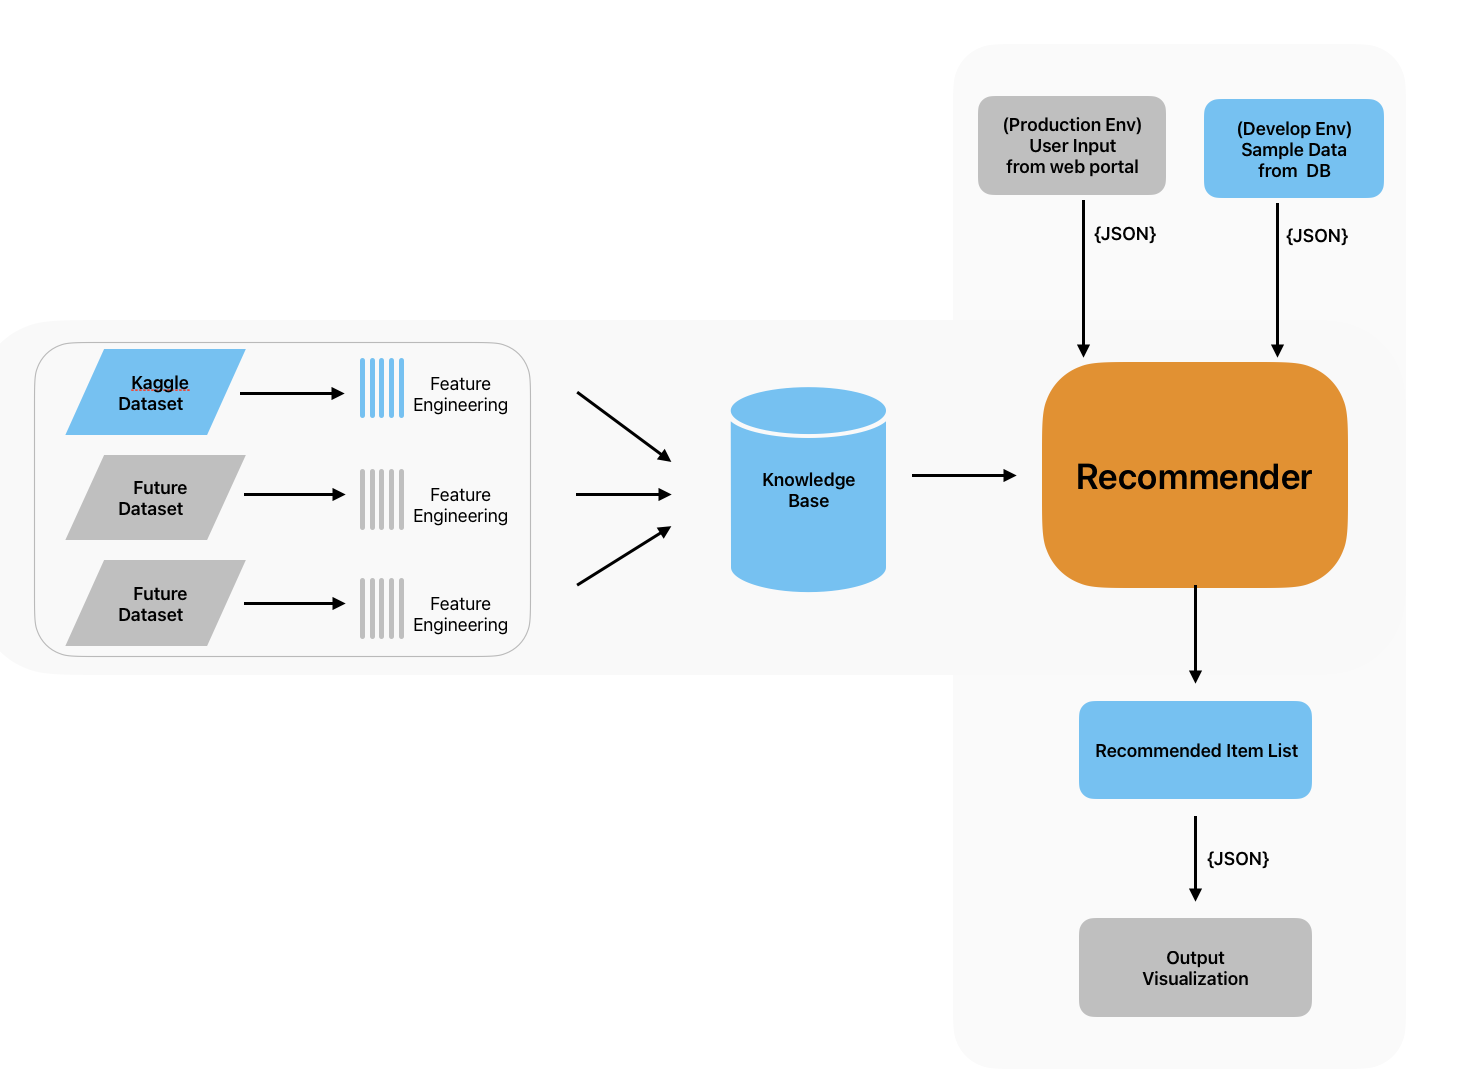
\includegraphics[width=0.8\textwidth,height=\textheight]{../image/2_solution_overview.png}

}

\end{figure}%

\subsection{Data Sources}\label{data-sources}

To support the development of our restaurant menu recommendation system,
we aggregate and validate data for two primary use cases:

\subsubsection{Input Data}\label{input-data}

\begin{figure}[H]

\caption{Input Data}

{\centering 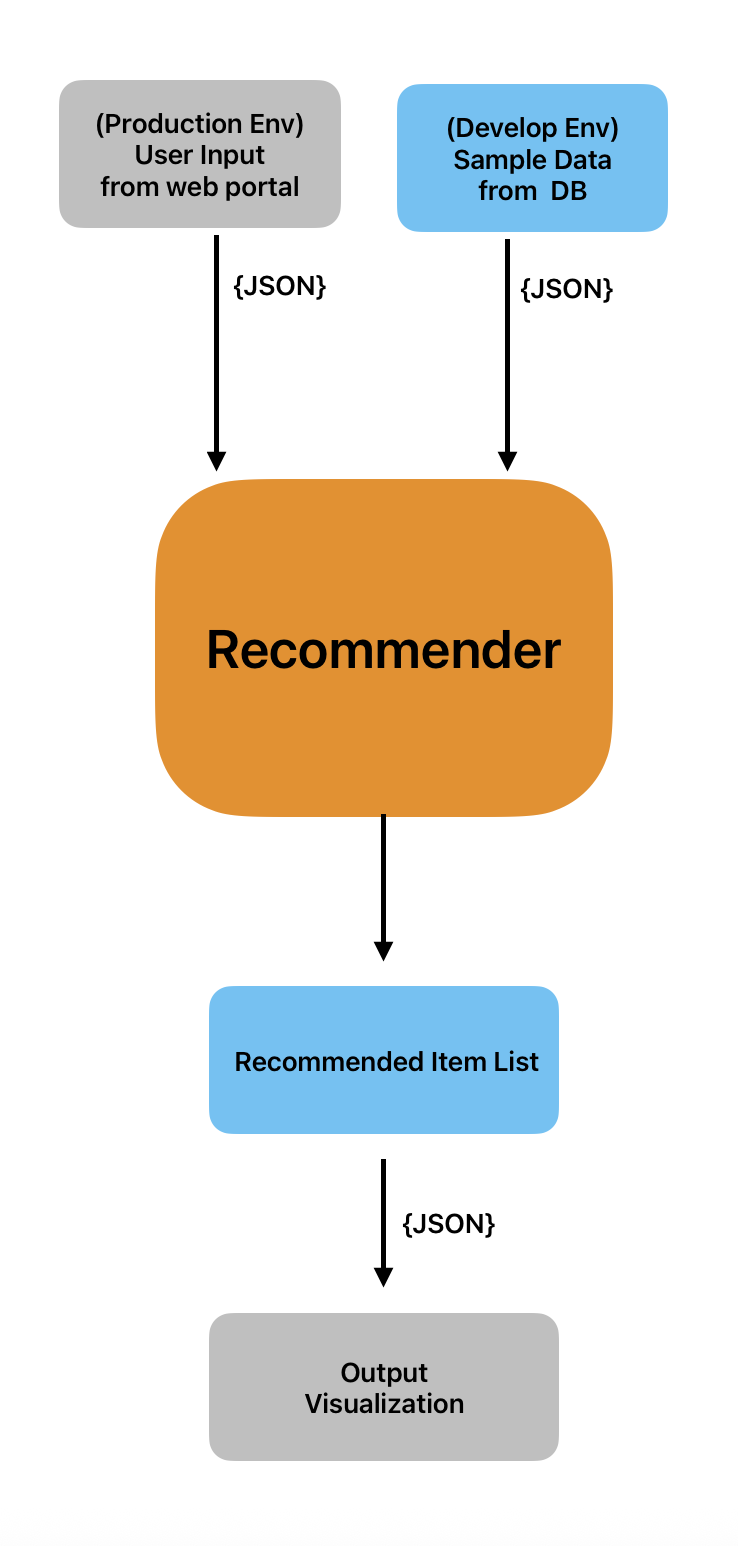
\includegraphics[width=0.3\textwidth,height=\textheight]{../image/3_input_data.png}

}

\end{figure}%

The internal Heymate database and user-submitted forms serve as
foundational inputs, providing:

\begin{itemize}
\tightlist
\item
  Restaurant Information: Name, Type, and Location\\
\item
  Menu Information: Item Name, Category, and Price
\end{itemize}

\subsubsection{Modelling Data}\label{modelling-data}

\begin{figure}

\caption{\label{fig-model-structure}Modelling Data}

\centering{

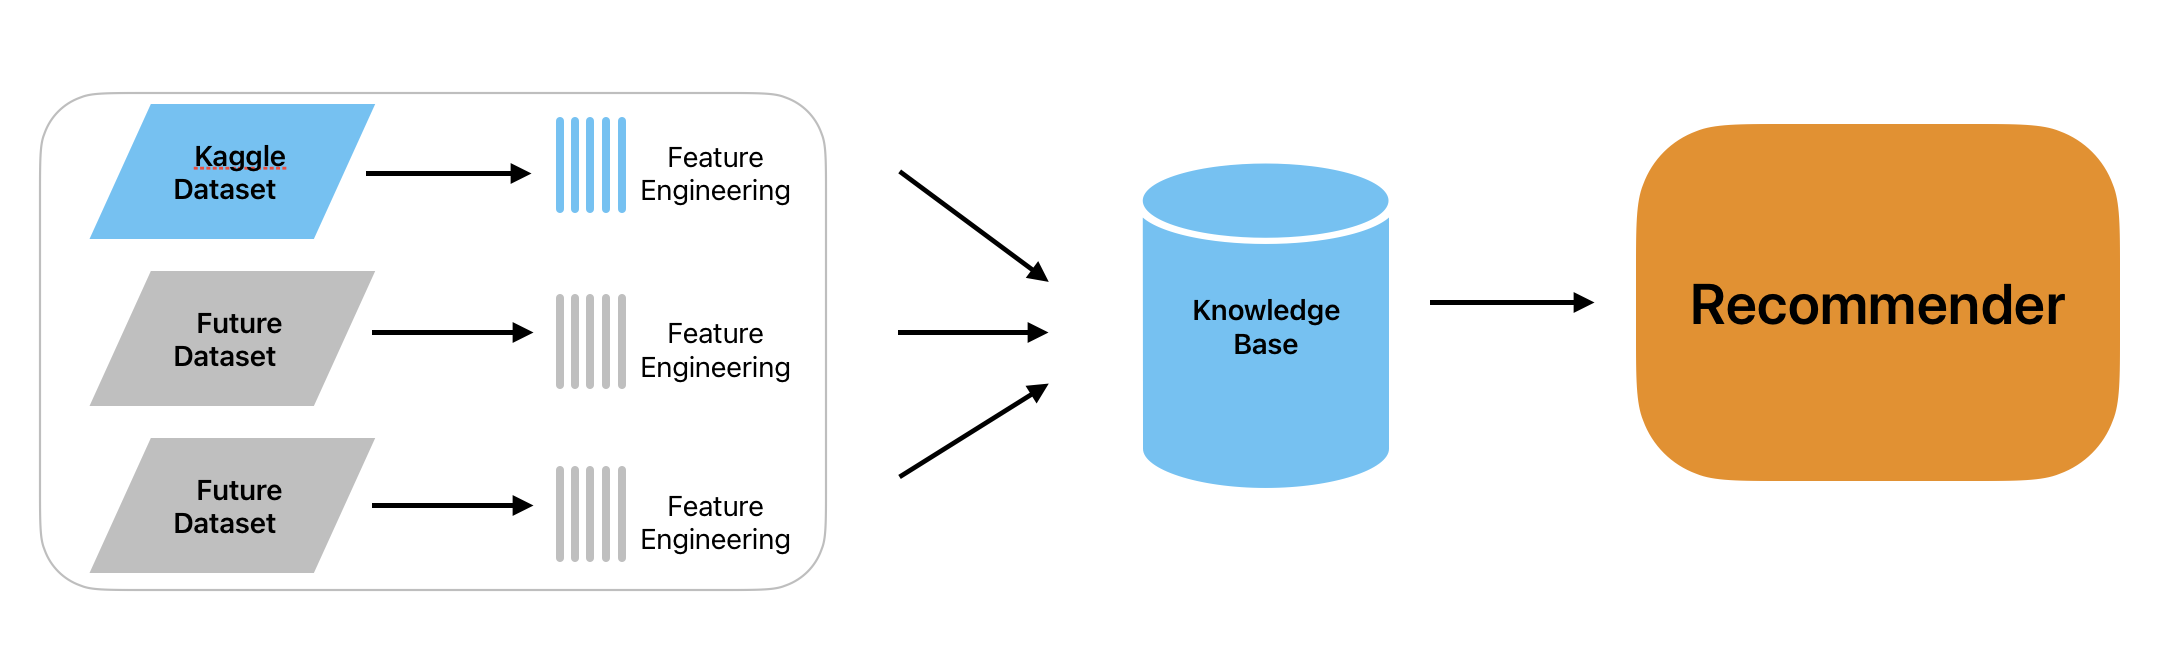
\includegraphics[width=0.8\textwidth,height=\textheight]{../image/4_modelling_data.png}

}

\end{figure}%

To enhance our understanding of menu popularity and strengthen the
foundation of our recommendation model, we plan to incorporate external
data sources including:

\begin{itemize}
\tightlist
\item
  Uber Eats USA Restaurants and Menus (Sakib (2024) from Kaggle): Offers
  modern restaurant-level data including ratings, menu items, and
  restaurant types
\item
  What's on the Menu? (Library (2016) from Kaggle): Provides historical
  menu data including item frequency, restaurant names, categories, and
  prices
\end{itemize}

\subsection{Data Validation (Initial
EDA)}\label{data-validation-initial-eda}

Our initial exploratory analysis revealed two key challenges that must
be addressed before modelling.

\subsubsection{Data Entry Challenge}\label{data-entry-challenge}

Menu item names are inconsistently formatted across restaurants as some
include item numbers, others use different naming styles or even
different languages. For example, the same dish may appear as ``Seafood
Fried Rice'', ``149. Fook Chow Seafood Fried Rice'', or a translated
version. These inconsistencies make it difficult to compare, group, or
analyze menu items reliably.

\begin{longtable}[]{@{}
  >{\raggedright\arraybackslash}p{(\columnwidth - 2\tabcolsep) * \real{0.6422}}
  >{\raggedright\arraybackslash}p{(\columnwidth - 2\tabcolsep) * \real{0.3578}}@{}}
\caption{Sample menu name from Heymate database}\tabularnewline
\toprule\noalign{}
\begin{minipage}[b]{\linewidth}\raggedright
ProductName
\end{minipage} & \begin{minipage}[b]{\linewidth}\raggedright
StoreName
\end{minipage} \\
\midrule\noalign{}
\endfirsthead
\toprule\noalign{}
\begin{minipage}[b]{\linewidth}\raggedright
ProductName
\end{minipage} & \begin{minipage}[b]{\linewidth}\raggedright
StoreName
\end{minipage} \\
\midrule\noalign{}
\endhead
\bottomrule\noalign{}
\endlastfoot
Seafood Fried Rice 魚蝦蟹炒飯 & Fisherman's Terrace \\
G25. Sauteed Seafood Fried Rice 避風塘海鮮炒飯 & Yue Ting Seafood
Restaurant \\
149. Fook Chow Seafood Fried Rice福州海皇炒饭 & Double Double Restaurant
\& Wonton Ltd. \\
160. XO Sauce W/ Seafood Fried Rice XO 酱海鲜炒饭 & Double Double
Restaurant \& Wonton Ltd. \\
161. Dried Scallop \& Seafood Fried Rice瑶柱海皇炒饭 & Double Double
Restaurant \& Wonton Ltd. \\
Seafood Fried Rice & Nishiki Sushi Bar \\
Assorted Seafood Fried Rice & So Good Restaurant \\
Seafood Fried Rice 鸿羊炒饭 & Fortune Lamb Dining \\
Seafood Fried Rice牛油海鮮炒飯 & Richmond \\
Seafood Fried Rice 海鮮炒飯 & Lougheed \\
Fu-Chow Style Seafood Fried Rice 福州炒飯 (Topped with sauce 有汁) &
Lougheed \\
Foo Chow Style Seafood Fried Rice / 福州炒飯 & Pelican Seafood
Restaurant \\
Seafood Fried Rice with Pineapple / 海鲜炒飯 & Pelican Seafood
Restaurant \\
Deluxe Seafood Fried Rice / 有米佬炒饭 & Pelican Seafood Restaurant \\
35. Seafood Fried Rice & Summer House \\
Seafood Fried Rice & Valendine \\
43.芝士白汁焗海鮮飯或意麵 Baked Creamy Seafood Fried Rice or Linguine &
Neptune Chinese Kitchen (UBC) \\
921. 福州瑤柱炒飯 Dried Scallop \& Mixed Seafood Fried Rice & Neptune
Chinese Kitchen (UBC) \\
926. 海鮮粒炒飯 Diced Mixed Seafood Fried Rice & Neptune Chinese Kitchen
(UBC) \\
3. Seafood Fried Rice Served In Whole Pineapple 原隻菠蘿船海鮮炒飯 &
Grand Crystal Seafood Restaurant \\
Seafood Fried Rice 海鲜炒饭 & Pinyuexuan Seafood Restaurant \\
931. 海鮮炒飯 Seafood Fried Rice & Lucky Fortune Seafood Restaurant \\
102. Fu-Chow Style Seafood Fried Rice 福州炒飯 & Lucky Fortune Seafood
Restaurant \\
\end{longtable}

To address this, we plan to leverage the capabilities of large language
models to clean and standardize menu item names. Inspired by industry
practices such as CloudKitchens' approach to multi-location menu
management (CloudKitchens (2024)), we will use GPT to:\\
- Normalize inconsistent item names\\
- Extract consistent tags

\begin{Shaded}
\begin{Highlighting}[]
\FunctionTok{\{}
  \DataTypeTok{"Base Item"}\FunctionTok{:} \StringTok{"Fried Rice"}\FunctionTok{,}
  \DataTypeTok{"Flavor Tag"}\FunctionTok{:} \StringTok{"Seafood"}
\FunctionTok{\}}
\end{Highlighting}
\end{Shaded}

\subsubsection{Modeling Challenge}\label{modeling-challenge}

A key challenge in our \hyperref[fig-model-structure]{modelling process}
is integrating multiple datasets that use inconsistent or non-standard
identifiers for restaurants and menu items.\\
To make these datasets work together, we need to:

\begin{itemize}
\tightlist
\item
  Align records using partially matching keys like restaurant and item
  names\\
\item
  Normalize variations in naming using LLMs\\
\item
  Enrich menu profiles by merging structured data from both sources,
  enabling robust popularity scoring
\end{itemize}

The final output is a unified and cleaned dataset enriched with relevant
features such as item frequency, price, and standardized names, laying
the groundwork for our Recommender Module.

\subsection{Recommender Module}\label{recommender-module}

\begin{figure}

\caption{\label{fig-visual-flow}Flow chart}

\centering{

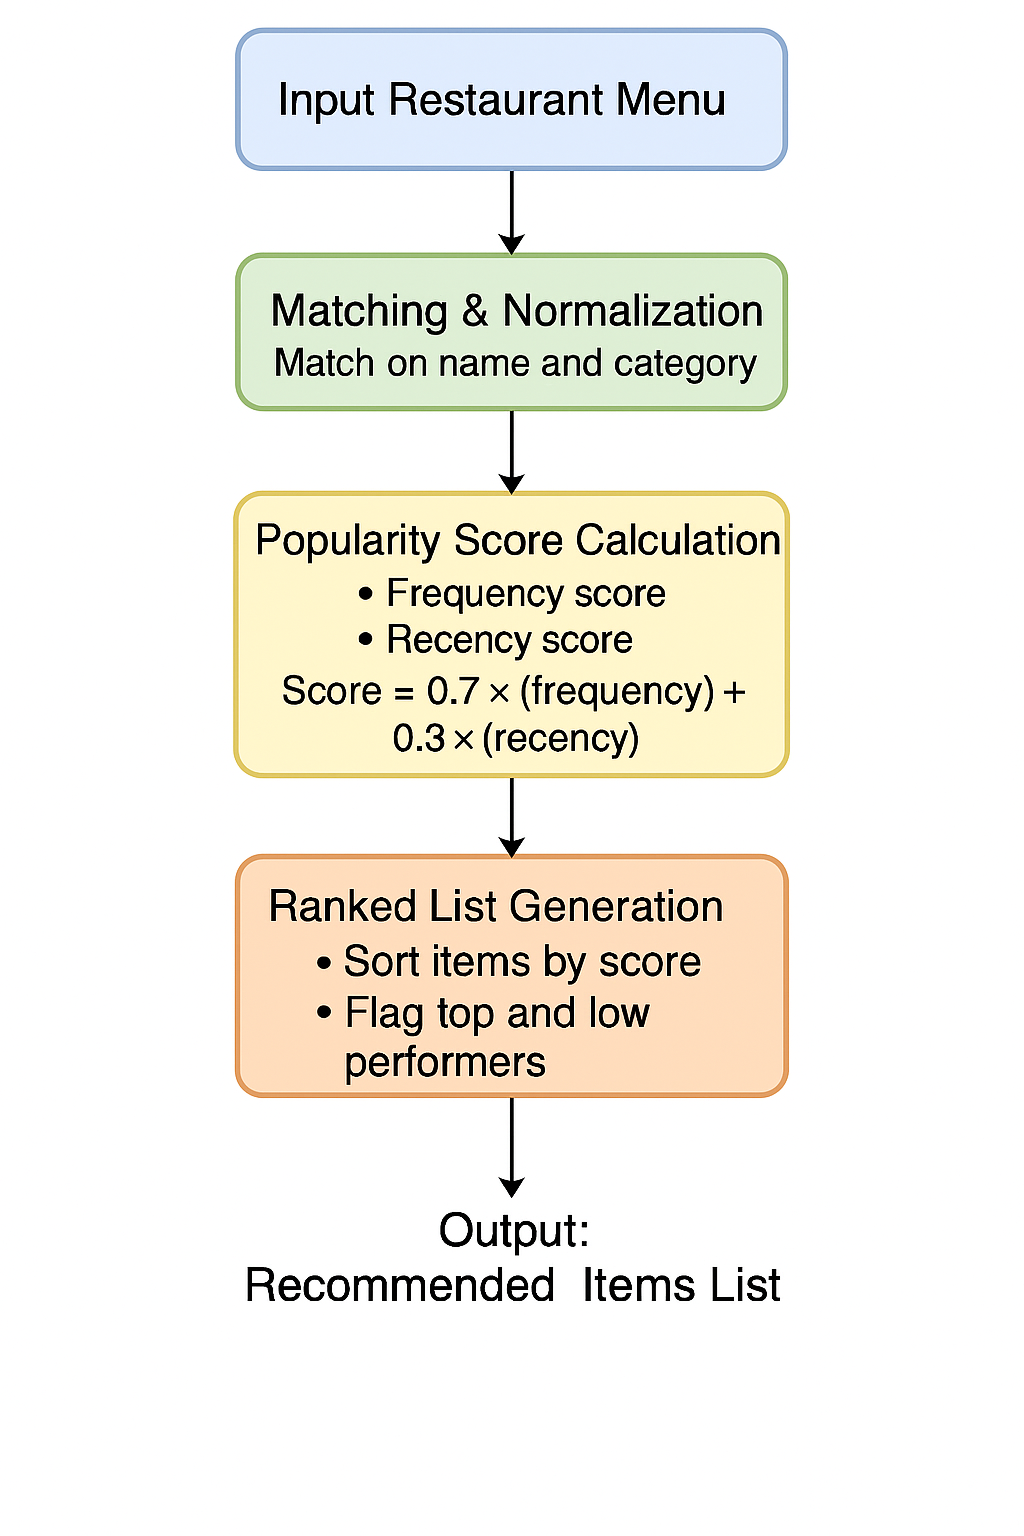
\includegraphics[width=0.4\textwidth,height=\textheight]{../image/1_visual_flow.png}

}

\end{figure}%

The recommender system operates through the following four steps as
shown in \hyperref[fig-visual-flow]{figure}:

\begin{enumerate}
\def\labelenumi{\arabic{enumi}.}
\item
  \textbf{Input Data Collection}

  \begin{itemize}
  \tightlist
  \item
    Restaurant Menu Data: A list of the restaurant's current menu items
    (names, categories, and optional descriptions).
  \item
    External Dataset: Built from the Kaggle menu dataset (and future
    sources), this captures broader market patterns such as how
    frequently and recently dishes appear across other restaurants.
  \end{itemize}
\item
  \textbf{Matching \& Normalization}\\
  The Menu item names vary widely across restaurants(e.g., ``BBQ Chicken
  Pizza'' vs ``Barbecue Chicken Pizza''). To address this:

  \begin{itemize}
  \tightlist
  \item
    We apply name normalization and category matching to link each
    restaurant's menu item to the closest equivalent in the knowledge
    base.
  \item
    To do this, we use a query-based matching approach that searches the
    knowledge base for the most similar items, even if names vary across
    restaurants.
  \item
    This enables alignment despite variations in wording or format.
  \end{itemize}
\item
  \textbf{Scoring}\\
  Once matched, each item receives a popularity score based on:

  \begin{itemize}
  \tightlist
  \item
    Frequency: How often the dish appears across menus in the dataset.
  \item
    Recency: How recently it has been featured
  \end{itemize}

  We use a weighted formula below to combine these factors:

  \textbf{Scoring formula:}\\
  \texttt{Score\ =\ 0.7\ ×\ (normalized\ frequency)\ +\ 0.3\ ×\ (normalized\ recency)}

  \textbf{Note:} These initial weights are heuristic and subject to
  refinement as we validate with partner feedback.
\item
  \textbf{Recommendation}\\
  After computing the popularity scores for each menu item, a ranked
  list to identify top and underperforming dishes is provided.
\end{enumerate}

\subsubsection{Example Use Case}\label{example-use-case}

Suppose a restaurant uploads its menu, which includes ``Hawaiian Pizza.
The recommender system: - Matches ``Hawaiian Pizza'' to its closest
entry in the knowledge base.\\
- Calculates its popularity score.\\
- Returns insights such as:\\
Popularity score: 62 (below market median)\\
It suggests adding trending dishes like ``BBQ Chicken Pizza'' that are
more popular.

\section{Final Data Product}\label{final-data-product}

Our solution is a menu recommendation engine and a simple visualization
demo, showing the top 20 popular items tailored to each restaurant. The
engine is powered by a query-based recommender trained on external
datasets. To simulate real-world use, we will test the tool using
historical data from Heymate's existing restaurant clients.

The anticipated business impact includes:

\begin{itemize}
\tightlist
\item
  Helping restaurant clients identify popular items, improve sales, and
  reduce waste\\
\item
  Supporting smarter menu decisions and client retention\\
\item
  Strengthening Heymate's value proposition as a data-driven platform
  partner
\end{itemize}

\subsection{Success Criteria}\label{success-criteria}

The project will be considered successful if internal tests using
Heymate's internal dataset sample produce results that align with
business expectations, and the visualization demo operates as intended.
Furthermore, the popularity scoring schema and recommender system will
be delivered as open-ended, modular components, enabling Heymate to
adapt and expand the solution in future development.

\section{Project Timeline}\label{project-timeline}

\begin{longtable}[]{@{}
  >{\raggedright\arraybackslash}p{(\columnwidth - 4\tabcolsep) * \real{0.2500}}
  >{\raggedright\arraybackslash}p{(\columnwidth - 4\tabcolsep) * \real{0.2500}}
  >{\raggedright\arraybackslash}p{(\columnwidth - 4\tabcolsep) * \real{0.5000}}@{}}
\toprule\noalign{}
\begin{minipage}[b]{\linewidth}\raggedright
Week
\end{minipage} & \begin{minipage}[b]{\linewidth}\raggedright
Date
\end{minipage} & \begin{minipage}[b]{\linewidth}\raggedright
Tasks
\end{minipage} \\
\midrule\noalign{}
\endhead
\bottomrule\noalign{}
\endlastfoot
Week 1 & May 5--9 & Proposal, Design Knowledge Base, Database setup \\
Week 2--4 & May 12--30 & LLM research and tuning, workspace setup, API
framework, core logic \\
Week 5 & June 2--5 & Integration and modularization \\
Week 6 & June 9--13 & Final review and report \\
\end{longtable}

\section{Appendices}\label{appendices}

\subsection{Addressing the Matching
Challenge}\label{addressing-the-matching-challenge}

Accurately matching menu items is one of the most challenging aspects
due to variability in naming conventions.\\
Initially, we will use query-based techniques such as string
normalization and category filtering.

To improve this process, we plan to explore pretrained models for
semantic matching, including:

\begin{itemize}
\tightlist
\item
  Sentence Transformers (SBERT)\\
\item
  spaCy similarity pipelines\\
\item
  FastText embeddings
\end{itemize}

These models will improve the ability to recognize and link creatively
named menu items to their standardized counterparts in the knowledge
base.

\newpage{}

\section*{References}\label{references}
\addcontentsline{toc}{section}{References}

\phantomsection\label{refs}
\begin{CSLReferences}{1}{0}
\bibitem[\citeproctext]{ref-cloudkitchens}
CloudKitchens. 2024. {``Multi-Channel, Multi-Location Menu
Management.''}
\url{https://techblog.cloudkitchens.com/p/multi-channel-multi-location-menu}.

\bibitem[\citeproctext]{ref-nypl2016menu}
Library, New York Public. 2016. {``What's on the Menu?''}
\url{https://www.kaggle.com/datasets/nypl/whats-on-the-menu}.

\bibitem[\citeproctext]{ref-sakib2023ubereats}
Sakib, Ahmed Shahriar. 2024. {``Uber Eats USA Restaurants \& Menus.''}
\url{https://www.kaggle.com/datasets/ahmedshahriarsakib/uber-eats-usa-restaurants-menus}.

\end{CSLReferences}




\end{document}
